% Options for packages loaded elsewhere
\PassOptionsToPackage{unicode}{hyperref}
\PassOptionsToPackage{hyphens}{url}
%
\documentclass[
]{article}
\usepackage{amsmath,amssymb}
\usepackage{lmodern}
\usepackage{iftex}
\ifPDFTeX
  \usepackage[T1]{fontenc}
  \usepackage[utf8]{inputenc}
  \usepackage{textcomp} % provide euro and other symbols
\else % if luatex or xetex
  \usepackage{unicode-math}
  \defaultfontfeatures{Scale=MatchLowercase}
  \defaultfontfeatures[\rmfamily]{Ligatures=TeX,Scale=1}
\fi
% Use upquote if available, for straight quotes in verbatim environments
\IfFileExists{upquote.sty}{\usepackage{upquote}}{}
\IfFileExists{microtype.sty}{% use microtype if available
  \usepackage[]{microtype}
  \UseMicrotypeSet[protrusion]{basicmath} % disable protrusion for tt fonts
}{}
\makeatletter
\@ifundefined{KOMAClassName}{% if non-KOMA class
  \IfFileExists{parskip.sty}{%
    \usepackage{parskip}
  }{% else
    \setlength{\parindent}{0pt}
    \setlength{\parskip}{6pt plus 2pt minus 1pt}}
}{% if KOMA class
  \KOMAoptions{parskip=half}}
\makeatother
\usepackage{xcolor}
\usepackage[margin=1in]{geometry}
\usepackage{color}
\usepackage{fancyvrb}
\newcommand{\VerbBar}{|}
\newcommand{\VERB}{\Verb[commandchars=\\\{\}]}
\DefineVerbatimEnvironment{Highlighting}{Verbatim}{commandchars=\\\{\}}
% Add ',fontsize=\small' for more characters per line
\usepackage{framed}
\definecolor{shadecolor}{RGB}{248,248,248}
\newenvironment{Shaded}{\begin{snugshade}}{\end{snugshade}}
\newcommand{\AlertTok}[1]{\textcolor[rgb]{0.94,0.16,0.16}{#1}}
\newcommand{\AnnotationTok}[1]{\textcolor[rgb]{0.56,0.35,0.01}{\textbf{\textit{#1}}}}
\newcommand{\AttributeTok}[1]{\textcolor[rgb]{0.77,0.63,0.00}{#1}}
\newcommand{\BaseNTok}[1]{\textcolor[rgb]{0.00,0.00,0.81}{#1}}
\newcommand{\BuiltInTok}[1]{#1}
\newcommand{\CharTok}[1]{\textcolor[rgb]{0.31,0.60,0.02}{#1}}
\newcommand{\CommentTok}[1]{\textcolor[rgb]{0.56,0.35,0.01}{\textit{#1}}}
\newcommand{\CommentVarTok}[1]{\textcolor[rgb]{0.56,0.35,0.01}{\textbf{\textit{#1}}}}
\newcommand{\ConstantTok}[1]{\textcolor[rgb]{0.00,0.00,0.00}{#1}}
\newcommand{\ControlFlowTok}[1]{\textcolor[rgb]{0.13,0.29,0.53}{\textbf{#1}}}
\newcommand{\DataTypeTok}[1]{\textcolor[rgb]{0.13,0.29,0.53}{#1}}
\newcommand{\DecValTok}[1]{\textcolor[rgb]{0.00,0.00,0.81}{#1}}
\newcommand{\DocumentationTok}[1]{\textcolor[rgb]{0.56,0.35,0.01}{\textbf{\textit{#1}}}}
\newcommand{\ErrorTok}[1]{\textcolor[rgb]{0.64,0.00,0.00}{\textbf{#1}}}
\newcommand{\ExtensionTok}[1]{#1}
\newcommand{\FloatTok}[1]{\textcolor[rgb]{0.00,0.00,0.81}{#1}}
\newcommand{\FunctionTok}[1]{\textcolor[rgb]{0.00,0.00,0.00}{#1}}
\newcommand{\ImportTok}[1]{#1}
\newcommand{\InformationTok}[1]{\textcolor[rgb]{0.56,0.35,0.01}{\textbf{\textit{#1}}}}
\newcommand{\KeywordTok}[1]{\textcolor[rgb]{0.13,0.29,0.53}{\textbf{#1}}}
\newcommand{\NormalTok}[1]{#1}
\newcommand{\OperatorTok}[1]{\textcolor[rgb]{0.81,0.36,0.00}{\textbf{#1}}}
\newcommand{\OtherTok}[1]{\textcolor[rgb]{0.56,0.35,0.01}{#1}}
\newcommand{\PreprocessorTok}[1]{\textcolor[rgb]{0.56,0.35,0.01}{\textit{#1}}}
\newcommand{\RegionMarkerTok}[1]{#1}
\newcommand{\SpecialCharTok}[1]{\textcolor[rgb]{0.00,0.00,0.00}{#1}}
\newcommand{\SpecialStringTok}[1]{\textcolor[rgb]{0.31,0.60,0.02}{#1}}
\newcommand{\StringTok}[1]{\textcolor[rgb]{0.31,0.60,0.02}{#1}}
\newcommand{\VariableTok}[1]{\textcolor[rgb]{0.00,0.00,0.00}{#1}}
\newcommand{\VerbatimStringTok}[1]{\textcolor[rgb]{0.31,0.60,0.02}{#1}}
\newcommand{\WarningTok}[1]{\textcolor[rgb]{0.56,0.35,0.01}{\textbf{\textit{#1}}}}
\usepackage{longtable,booktabs,array}
\usepackage{calc} % for calculating minipage widths
% Correct order of tables after \paragraph or \subparagraph
\usepackage{etoolbox}
\makeatletter
\patchcmd\longtable{\par}{\if@noskipsec\mbox{}\fi\par}{}{}
\makeatother
% Allow footnotes in longtable head/foot
\IfFileExists{footnotehyper.sty}{\usepackage{footnotehyper}}{\usepackage{footnote}}
\makesavenoteenv{longtable}
\usepackage{graphicx}
\makeatletter
\def\maxwidth{\ifdim\Gin@nat@width>\linewidth\linewidth\else\Gin@nat@width\fi}
\def\maxheight{\ifdim\Gin@nat@height>\textheight\textheight\else\Gin@nat@height\fi}
\makeatother
% Scale images if necessary, so that they will not overflow the page
% margins by default, and it is still possible to overwrite the defaults
% using explicit options in \includegraphics[width, height, ...]{}
\setkeys{Gin}{width=\maxwidth,height=\maxheight,keepaspectratio}
% Set default figure placement to htbp
\makeatletter
\def\fps@figure{htbp}
\makeatother
\setlength{\emergencystretch}{3em} % prevent overfull lines
\providecommand{\tightlist}{%
  \setlength{\itemsep}{0pt}\setlength{\parskip}{0pt}}
\setcounter{secnumdepth}{-\maxdimen} % remove section numbering
\usepackage{booktabs}
\usepackage{longtable}
\usepackage{array}
\usepackage{multirow}
\usepackage{wrapfig}
\usepackage{float}
\usepackage{colortbl}
\usepackage{pdflscape}
\usepackage{tabu}
\usepackage{threeparttable}
\usepackage{threeparttablex}
\usepackage[normalem]{ulem}
\usepackage{makecell}
\usepackage{xcolor}
\ifLuaTeX
  \usepackage{selnolig}  % disable illegal ligatures
\fi
\IfFileExists{bookmark.sty}{\usepackage{bookmark}}{\usepackage{hyperref}}
\IfFileExists{xurl.sty}{\usepackage{xurl}}{} % add URL line breaks if available
\urlstyle{same} % disable monospaced font for URLs
\hypersetup{
  pdftitle={Project},
  pdfauthor={Trinath Sai Subhash Reddy Pittala, Uma Maheswara R Meleti, Hemanth Vasireddy},
  hidelinks,
  pdfcreator={LaTeX via pandoc}}

\title{Project}
\author{Trinath Sai Subhash Reddy Pittala, Uma Maheswara R Meleti,
Hemanth Vasireddy}
\date{2023-03-24}

\begin{document}
\maketitle

\hypertarget{introduction}{%
\section{Introduction}\label{introduction}}

\hypertarget{airbnb-price-determinants-in-europe}{%
\subsection{Airbnb Price Determinants in
Europe}\label{airbnb-price-determinants-in-europe}}

We want to work on Airbnb's dataset from kaggle.com. It provides
information about hotel rooms in Europe.

Each major city has its dataset for weekends and weekdays Variables
included in the dataset: Host ID (Id) The total price of listing
(realSum) Room type: private, shared, entire home, apt (room\_type)
Whether or not a room is shared (room\_shared) Max number of people
allowed in property (person\_capacity) Whether or not the host is
superhost (host\_is\_superhost) Whether or not it is multiple rooms
(multi) Whether for business or family use (biz) Distance from the city
center (dist) Distance from nearest metro (metro\_dist) Latitude and
longitude (lat long) Guest satisfaction (guest\_satisfaction\_overall)
Cleanliness (cleanliness\_rating) The total quantity of bedrooms
available among all properties for a single host (bedrooms)

Questions we can answer with the dataset: Price Forecasting: use
pricing, room type, and amenities to predict potential rental prices in
the future. Hotspots: use listing location in relation to business and
tourism centers and correlate this with pricing to determine where
Airbnb rentals would be most profitable Customer sentiment analysis:
analyze customer comments and satisfaction ratings to evaluate listing
on overall customer experience and use it to optimize hosts' services to
improve user satisfaction ratings.

How can this information be used: Data can help travelers find
accommodation that meets their needs without exceeding budget. Can help
hosts set competitive pricing and optimize listings to get more
bookings. Help investors evaluate the value of investing in real estate
in different European cities based on pricing trends.

\hypertarget{pre-processing-and-cleaning-the-data}{%
\section{Pre Processing and Cleaning the
Data}\label{pre-processing-and-cleaning-the-data}}

\hypertarget{data-loading}{%
\subsection{Data loading}\label{data-loading}}

\begin{Shaded}
\begin{Highlighting}[]
\CommentTok{\# Set the relative directory path}
\NormalTok{my\_dir }\OtherTok{\textless{}{-}} \StringTok{"./archive"}

\CommentTok{\# List all the files in the directory}
\NormalTok{files }\OtherTok{\textless{}{-}} \FunctionTok{list.files}\NormalTok{(}\AttributeTok{path =}\NormalTok{ my\_dir, }\AttributeTok{full.names =} \ConstantTok{TRUE}\NormalTok{)}
\end{Highlighting}
\end{Shaded}

\hypertarget{combining-the-data-from-all-files}{%
\subsubsection{Combining the Data from all
Files}\label{combining-the-data-from-all-files}}

\begin{Shaded}
\begin{Highlighting}[]
\CommentTok{\# Get a list of all the csv files in the directory}
\NormalTok{file\_list }\OtherTok{\textless{}{-}} \FunctionTok{list.files}\NormalTok{(}\AttributeTok{path =}\NormalTok{ my\_dir, }\AttributeTok{pattern =} \StringTok{"*.csv"}\NormalTok{, }\AttributeTok{full.names =} \ConstantTok{TRUE}\NormalTok{)}

\CommentTok{\# Initialize an empty list to store the data frames}
\NormalTok{df\_list }\OtherTok{\textless{}{-}} \FunctionTok{list}\NormalTok{()}

\CommentTok{\# Loop through each file and read it into a data frame}
\ControlFlowTok{for}\NormalTok{ (i }\ControlFlowTok{in} \FunctionTok{seq\_along}\NormalTok{(file\_list)) \{}
\NormalTok{    df }\OtherTok{\textless{}{-}} \FunctionTok{read.csv}\NormalTok{(file\_list[i])}

    \CommentTok{\# Add a new column with the city\_day}
\NormalTok{    df}\SpecialCharTok{$}\NormalTok{city\_day }\OtherTok{\textless{}{-}} \FunctionTok{basename}\NormalTok{(file\_list[i])}

    \CommentTok{\# Append the data frame to the list}
\NormalTok{    df\_list[[i]] }\OtherTok{\textless{}{-}}\NormalTok{ df}
\NormalTok{\}}

\CommentTok{\# Combine all the data frames into a single dataset}
\NormalTok{my\_data }\OtherTok{\textless{}{-}} \FunctionTok{bind\_rows}\NormalTok{(df\_list)}

\CommentTok{\# Removing the .csv ext}
\NormalTok{my\_data}\SpecialCharTok{$}\NormalTok{city\_day }\OtherTok{\textless{}{-}} \FunctionTok{gsub}\NormalTok{(}\StringTok{"}\SpecialCharTok{\textbackslash{}\textbackslash{}}\StringTok{.csv"}\NormalTok{, }\StringTok{""}\NormalTok{, my\_data}\SpecialCharTok{$}\NormalTok{city\_day)}

\CommentTok{\# Print the first few rows of the data}
\FunctionTok{head}\NormalTok{(my\_data)}
\end{Highlighting}
\end{Shaded}

\begin{verbatim}
##   X  realSum    room_type room_shared room_private person_capacity
## 1 0 194.0337 Private room       False         True               2
## 2 1 344.2458 Private room       False         True               4
## 3 2 264.1014 Private room       False         True               2
## 4 3 433.5294 Private room       False         True               4
## 5 4 485.5529 Private room       False         True               2
## 6 5 552.8086 Private room       False         True               3
##   host_is_superhost multi biz cleanliness_rating guest_satisfaction_overall
## 1             False     1   0                 10                         93
## 2             False     0   0                  8                         85
## 3             False     0   1                  9                         87
## 4             False     0   1                  9                         90
## 5              True     0   0                 10                         98
## 6             False     0   0                  8                        100
##   bedrooms      dist metro_dist attr_index attr_index_norm rest_index
## 1        1 5.0229638  2.5393800   78.69038        4.166708   98.25390
## 2        1 0.4883893  0.2394039  631.17638       33.421209  837.28076
## 3        1 5.7483119  3.6516213   75.27588        3.985908   95.38695
## 4        2 0.3848620  0.4398761  493.27253       26.119108  875.03310
## 5        1 0.5447382  0.3186926  552.83032       29.272733  815.30574
## 6        2 2.1314201  1.9046682  174.78896        9.255191  225.20166
##   rest_index_norm     lng      lat           city_day
## 1        6.846473 4.90569 52.41772 amsterdam_weekdays
## 2       58.342928 4.90005 52.37432 amsterdam_weekdays
## 3        6.646700 4.97512 52.36103 amsterdam_weekdays
## 4       60.973565 4.89417 52.37663 amsterdam_weekdays
## 5       56.811677 4.90051 52.37508 amsterdam_weekdays
## 6       15.692376 4.87699 52.38966 amsterdam_weekdays
\end{verbatim}

\hypertarget{spilt-training-and-testing-data}{%
\subsubsection{Spilt Training and Testing
Data}\label{spilt-training-and-testing-data}}

\begin{Shaded}
\begin{Highlighting}[]
\FunctionTok{set.seed}\NormalTok{(}\DecValTok{123456789}\NormalTok{)}
\NormalTok{my\_data\_train }\OtherTok{\textless{}{-}}\NormalTok{ my\_data[}\FunctionTok{sample}\NormalTok{(}\FunctionTok{nrow}\NormalTok{(my\_data), }\FloatTok{0.7} \SpecialCharTok{*} \FunctionTok{nrow}\NormalTok{(my\_data)),}
\NormalTok{    ]}
\NormalTok{my\_data\_test }\OtherTok{\textless{}{-}}\NormalTok{ my\_data[}\FunctionTok{setdiff}\NormalTok{(}\DecValTok{1}\SpecialCharTok{:}\FunctionTok{nrow}\NormalTok{(my\_data), }\FunctionTok{rownames}\NormalTok{(my\_data\_train)),}
\NormalTok{    ]}
\FunctionTok{head}\NormalTok{(my\_data\_train)}
\end{Highlighting}
\end{Shaded}

\begin{verbatim}
##          X  realSum       room_type room_shared room_private person_capacity
## 44098  462 368.6905 Entire home/apt       False        False               4
## 47120 3484 240.3385 Entire home/apt       False        False               4
## 29708 2631 257.7671    Private room       False         True               2
## 9772   856 485.9543 Entire home/apt       False        False               2
## 16896  196 269.4653 Entire home/apt       False        False               4
## 2325   244 220.2798 Entire home/apt       False        False               6
##       host_is_superhost multi biz cleanliness_rating guest_satisfaction_overall
## 44098             False     0   1                  8                         80
## 47120             False     0   1                  8                        100
## 29708             False     0   0                 10                        100
## 9772              False     0   0                  9                         84
## 16896             False     0   1                 10                         93
## 2325              False     1   0                 10                         98
##       bedrooms      dist metro_dist attr_index attr_index_norm rest_index
## 44098        1 1.4966090  0.5553737 1758.54461       38.961335  2076.9803
## 47120        1 2.7716179  0.5800582  574.88024       12.736727  1479.5874
## 29708        1 6.5817328  2.0478099  172.41005       11.984895   385.5078
## 9772         1 1.0793735  0.3433846  472.88903       18.258792  1141.3205
## 16896        1 0.8901721  0.5452364  339.08856       11.194767   684.5563
## 2325         3 2.0502381  0.5606083   74.35373        2.803444   107.7512
##       rest_index_norm      lng      lat           city_day
## 44098       45.252362 12.48423 41.90030      rome_weekends
## 47120       32.236620 12.46991 41.90711      rome_weekends
## 29708        6.899917 -0.18190 51.45989    london_weekends
## 9772        25.070976  2.16725 41.37764 barcelona_weekends
## 16896       30.615911 -9.12964 38.71413    lisbon_weekdays
## 2325         8.090617 23.75717 37.98218    athens_weekdays
\end{verbatim}

\begin{Shaded}
\begin{Highlighting}[]
\FunctionTok{head}\NormalTok{(my\_data\_test)}
\end{Highlighting}
\end{Shaded}

\begin{verbatim}
##     X  realSum       room_type room_shared room_private person_capacity
## 3   2 264.1014    Private room       False         True               2
## 4   3 433.5294    Private room       False         True               4
## 10  9 276.5215    Private room       False         True               2
## 12 11 319.6401    Private room       False         True               2
## 17 16 368.8515    Private room       False         True               2
## 22 21 933.8458 Entire home/apt       False        False               4
##    host_is_superhost multi biz cleanliness_rating guest_satisfaction_overall
## 3              False     0   1                  9                         87
## 4              False     0   1                  9                         90
## 10             False     1   0                 10                         88
## 12              True     1   0                 10                         97
## 17             False     0   0                 10                         90
## 22             False     0   0                 10                         96
##    bedrooms     dist metro_dist attr_index attr_index_norm rest_index
## 3         1 5.748312  3.6516213   75.27588        3.985908   95.38695
## 4         2 0.384862  0.4398761  493.27253       26.119108  875.03310
## 10        1 3.142361  0.9244044  206.25286       10.921226  238.29126
## 12        1 2.182707  1.5903814  191.50134       10.140123  229.29740
## 17        1 1.327797  0.1195281  539.01288       28.541090  573.89657
## 22        2 1.014066  0.3771037  477.79407       25.299513  664.05325
##    rest_index_norm     lng      lat           city_day
## 3          6.64670 4.97512 52.36103 amsterdam_weekdays
## 4         60.97357 4.89417 52.37663 amsterdam_weekdays
## 10        16.60448 4.87600 52.34700 amsterdam_weekdays
## 12        15.97777 4.92496 52.37107 amsterdam_weekdays
## 17        39.98994 4.88971 52.36148 amsterdam_weekdays
## 22        46.27219 4.89088 52.36422 amsterdam_weekdays
\end{verbatim}

\hypertarget{filtering-out-the-outliers-from-data-out-of-iqr-ranges}{%
\subsubsection{Filtering out the Outliers from Data Out of IQR
Ranges}\label{filtering-out-the-outliers-from-data-out-of-iqr-ranges}}

\begin{Shaded}
\begin{Highlighting}[]
\CommentTok{\# Initialize an empty list to store the outliers}
\NormalTok{outliers\_list }\OtherTok{\textless{}{-}} \FunctionTok{list}\NormalTok{()}

\CommentTok{\# Initialize an empty list to store the filtered data}
\CommentTok{\# frames}
\NormalTok{df\_list\_filtered }\OtherTok{\textless{}{-}} \FunctionTok{list}\NormalTok{()}

\CommentTok{\# Loop through each file and read it into a data frame}
\CommentTok{\# after removing outliers}
\ControlFlowTok{for}\NormalTok{ (i }\ControlFlowTok{in} \FunctionTok{seq\_along}\NormalTok{(file\_list)) \{}
\NormalTok{    df\_filtered }\OtherTok{\textless{}{-}} \FunctionTok{read.csv}\NormalTok{(file\_list[i])}

    \CommentTok{\# Add a new column with the city\_day}
\NormalTok{    df\_filtered}\SpecialCharTok{$}\NormalTok{city\_day }\OtherTok{\textless{}{-}} \FunctionTok{gsub}\NormalTok{(}\StringTok{"}\SpecialCharTok{\textbackslash{}\textbackslash{}}\StringTok{.csv"}\NormalTok{, }\StringTok{""}\NormalTok{, }\FunctionTok{basename}\NormalTok{(file\_list[i]))}

\NormalTok{    iqr\_var1 }\OtherTok{\textless{}{-}} \FunctionTok{IQR}\NormalTok{(df\_filtered}\SpecialCharTok{$}\NormalTok{realSum)}

    \CommentTok{\# Calculate the upper and lower bounds for each}
    \CommentTok{\# variable}
\NormalTok{    upper\_var1 }\OtherTok{\textless{}{-}} \FunctionTok{quantile}\NormalTok{(df\_filtered}\SpecialCharTok{$}\NormalTok{realSum, }\FloatTok{0.75}\NormalTok{) }\SpecialCharTok{+} \FloatTok{1.5} \SpecialCharTok{*}
\NormalTok{        iqr\_var1}
\NormalTok{    lower\_var1 }\OtherTok{\textless{}{-}} \FunctionTok{quantile}\NormalTok{(df\_filtered}\SpecialCharTok{$}\NormalTok{realSum, }\FloatTok{0.25}\NormalTok{) }\SpecialCharTok{{-}} \FloatTok{1.5} \SpecialCharTok{*}
\NormalTok{        iqr\_var1}

    \CommentTok{\# Filter the data based on the upper and lower bounds}
    \CommentTok{\# for each variable}
\NormalTok{    filtered\_data }\OtherTok{\textless{}{-}} \FunctionTok{filter}\NormalTok{(df\_filtered, realSum }\SpecialCharTok{\textgreater{}}\NormalTok{ lower\_var1 }\SpecialCharTok{\&}
\NormalTok{        realSum }\SpecialCharTok{\textless{}}\NormalTok{ upper\_var1)}

    \CommentTok{\# Append the filtered data frame to the list}
\NormalTok{    df\_list\_filtered[[i]] }\OtherTok{\textless{}{-}}\NormalTok{ filtered\_data}

    \CommentTok{\# Get the rows that were removed while filtering}
\NormalTok{    outliers }\OtherTok{\textless{}{-}} \FunctionTok{anti\_join}\NormalTok{(df\_filtered, filtered\_data)}

    \CommentTok{\# Append the outliers to the list}
\NormalTok{    outliers\_list[[i]] }\OtherTok{\textless{}{-}}\NormalTok{ outliers}
\NormalTok{\}}


\CommentTok{\# Combine all the filtered data frames into a single}
\CommentTok{\# dataset}
\NormalTok{my\_data\_filtered }\OtherTok{\textless{}{-}} \FunctionTok{bind\_rows}\NormalTok{(df\_list\_filtered)}

\CommentTok{\# Removing the .csv ext}
\NormalTok{my\_data\_filtered}\SpecialCharTok{$}\NormalTok{city\_day }\OtherTok{\textless{}{-}} \FunctionTok{gsub}\NormalTok{(}\StringTok{"}\SpecialCharTok{\textbackslash{}\textbackslash{}}\StringTok{.csv"}\NormalTok{, }\StringTok{""}\NormalTok{, my\_data\_filtered}\SpecialCharTok{$}\NormalTok{city\_day)}

\CommentTok{\# summary(my\_data\_filtered)}

\CommentTok{\# Combine all the outliers into a single dataset}
\NormalTok{my\_outliers }\OtherTok{\textless{}{-}} \FunctionTok{bind\_rows}\NormalTok{(outliers\_list)}

\CommentTok{\# Removing the .csv ext}
\NormalTok{my\_outliers}\SpecialCharTok{$}\NormalTok{city\_day }\OtherTok{\textless{}{-}} \FunctionTok{gsub}\NormalTok{(}\StringTok{"}\SpecialCharTok{\textbackslash{}\textbackslash{}}\StringTok{.csv"}\NormalTok{, }\StringTok{""}\NormalTok{, my\_outliers}\SpecialCharTok{$}\NormalTok{city\_day)}

\FunctionTok{summary}\NormalTok{(my\_outliers)}
\end{Highlighting}
\end{Shaded}

\begin{verbatim}
##        X           realSum         room_type         room_shared       
##  Min.   :   0   Min.   :  279.4   Length:2737        Length:2737       
##  1st Qu.: 666   1st Qu.:  469.2   Class :character   Class :character  
##  Median :1237   Median :  691.9   Mode  :character   Mode  :character  
##  Mean   :1614   Mean   :  915.5                                        
##  3rd Qu.:2310   3rd Qu.:  996.3                                        
##  Max.   :5374   Max.   :18545.5                                        
##  room_private       person_capacity host_is_superhost      multi      
##  Length:2737        Min.   :2.000   Length:2737        Min.   :0.000  
##  Class :character   1st Qu.:4.000   Class :character   1st Qu.:0.000  
##  Mode  :character   Median :5.000   Mode  :character   Median :0.000  
##                     Mean   :4.628                      Mean   :0.221  
##                     3rd Qu.:6.000                      3rd Qu.:0.000  
##                     Max.   :6.000                      Max.   :1.000  
##       biz         cleanliness_rating guest_satisfaction_overall    bedrooms    
##  Min.   :0.0000   Min.   : 2.000     Min.   : 20.00             Min.   :0.000  
##  1st Qu.:0.0000   1st Qu.: 9.000     1st Qu.: 91.00             1st Qu.:1.000  
##  Median :0.0000   Median :10.000     Median : 97.00             Median :2.000  
##  Mean   :0.4965   Mean   : 9.509     Mean   : 93.65             Mean   :1.886  
##  3rd Qu.:1.0000   3rd Qu.:10.000     3rd Qu.:100.00             3rd Qu.:2.000  
##  Max.   :1.0000   Max.   :10.000     Max.   :100.00             Max.   :6.000  
##       dist            metro_dist         attr_index     attr_index_norm  
##  Min.   : 0.01504   Min.   :0.006171   Min.   :  20.5   Min.   :  1.468  
##  1st Qu.: 1.04119   1st Qu.:0.218081   1st Qu.: 225.1   1st Qu.: 11.719  
##  Median : 1.89579   Median :0.352339   Median : 385.0   Median : 17.958  
##  Mean   : 2.30674   Mean   :0.498426   Mean   : 456.2   Mean   : 20.892  
##  3rd Qu.: 3.00820   3rd Qu.:0.576430   3rd Qu.: 610.6   3rd Qu.: 25.953  
##  Max.   :21.29515   Max.   :8.918036   Max.   :2040.4   Max.   :100.000  
##    rest_index     rest_index_norm        lng                lat       
##  Min.   :  27.9   Min.   :  0.667   Min.   :-9.22476   Min.   :37.96  
##  1st Qu.: 408.5   1st Qu.: 14.187   1st Qu.:-0.06677   1st Qu.:41.41  
##  Median : 739.9   Median : 30.001   Median : 4.88384   Median :47.51  
##  Mean   : 904.9   Mean   : 31.734   Mean   : 7.88764   Mean   :45.93  
##  3rd Qu.:1269.7   3rd Qu.: 45.426   3rd Qu.:13.44666   3rd Qu.:51.50  
##  Max.   :4183.1   Max.   :100.000   Max.   :23.75400   Max.   :52.58  
##    city_day        
##  Length:2737       
##  Class :character  
##  Mode  :character  
##                    
##                    
## 
\end{verbatim}

\hypertarget{exploratory-data-analysis}{%
\section{Exploratory Data Analysis}\label{exploratory-data-analysis}}

\hypertarget{boxplot-of-price-vs-city}{%
\subsubsection{Boxplot of Price Vs
City}\label{boxplot-of-price-vs-city}}

\begin{Shaded}
\begin{Highlighting}[]
\FunctionTok{ggplot}\NormalTok{(my\_data\_filtered, }\FunctionTok{aes}\NormalTok{(}\AttributeTok{x =} \FunctionTok{reorder}\NormalTok{(city\_day, realSum, }\AttributeTok{FUN =}\NormalTok{ median),}
    \AttributeTok{y =}\NormalTok{ realSum, }\AttributeTok{fill =}\NormalTok{ city\_day)) }\SpecialCharTok{+} \FunctionTok{geom\_boxplot}\NormalTok{() }\SpecialCharTok{+} \FunctionTok{coord\_flip}\NormalTok{() }\SpecialCharTok{+}
    \FunctionTok{theme}\NormalTok{(}\AttributeTok{legend.key.height =} \FunctionTok{unit}\NormalTok{(}\FloatTok{0.5}\NormalTok{, }\StringTok{"cm"}\NormalTok{), }\AttributeTok{legend.key.size =} \FunctionTok{unit}\NormalTok{(}\DecValTok{1}\NormalTok{,}
        \StringTok{"lines"}\NormalTok{))}
\end{Highlighting}
\end{Shaded}

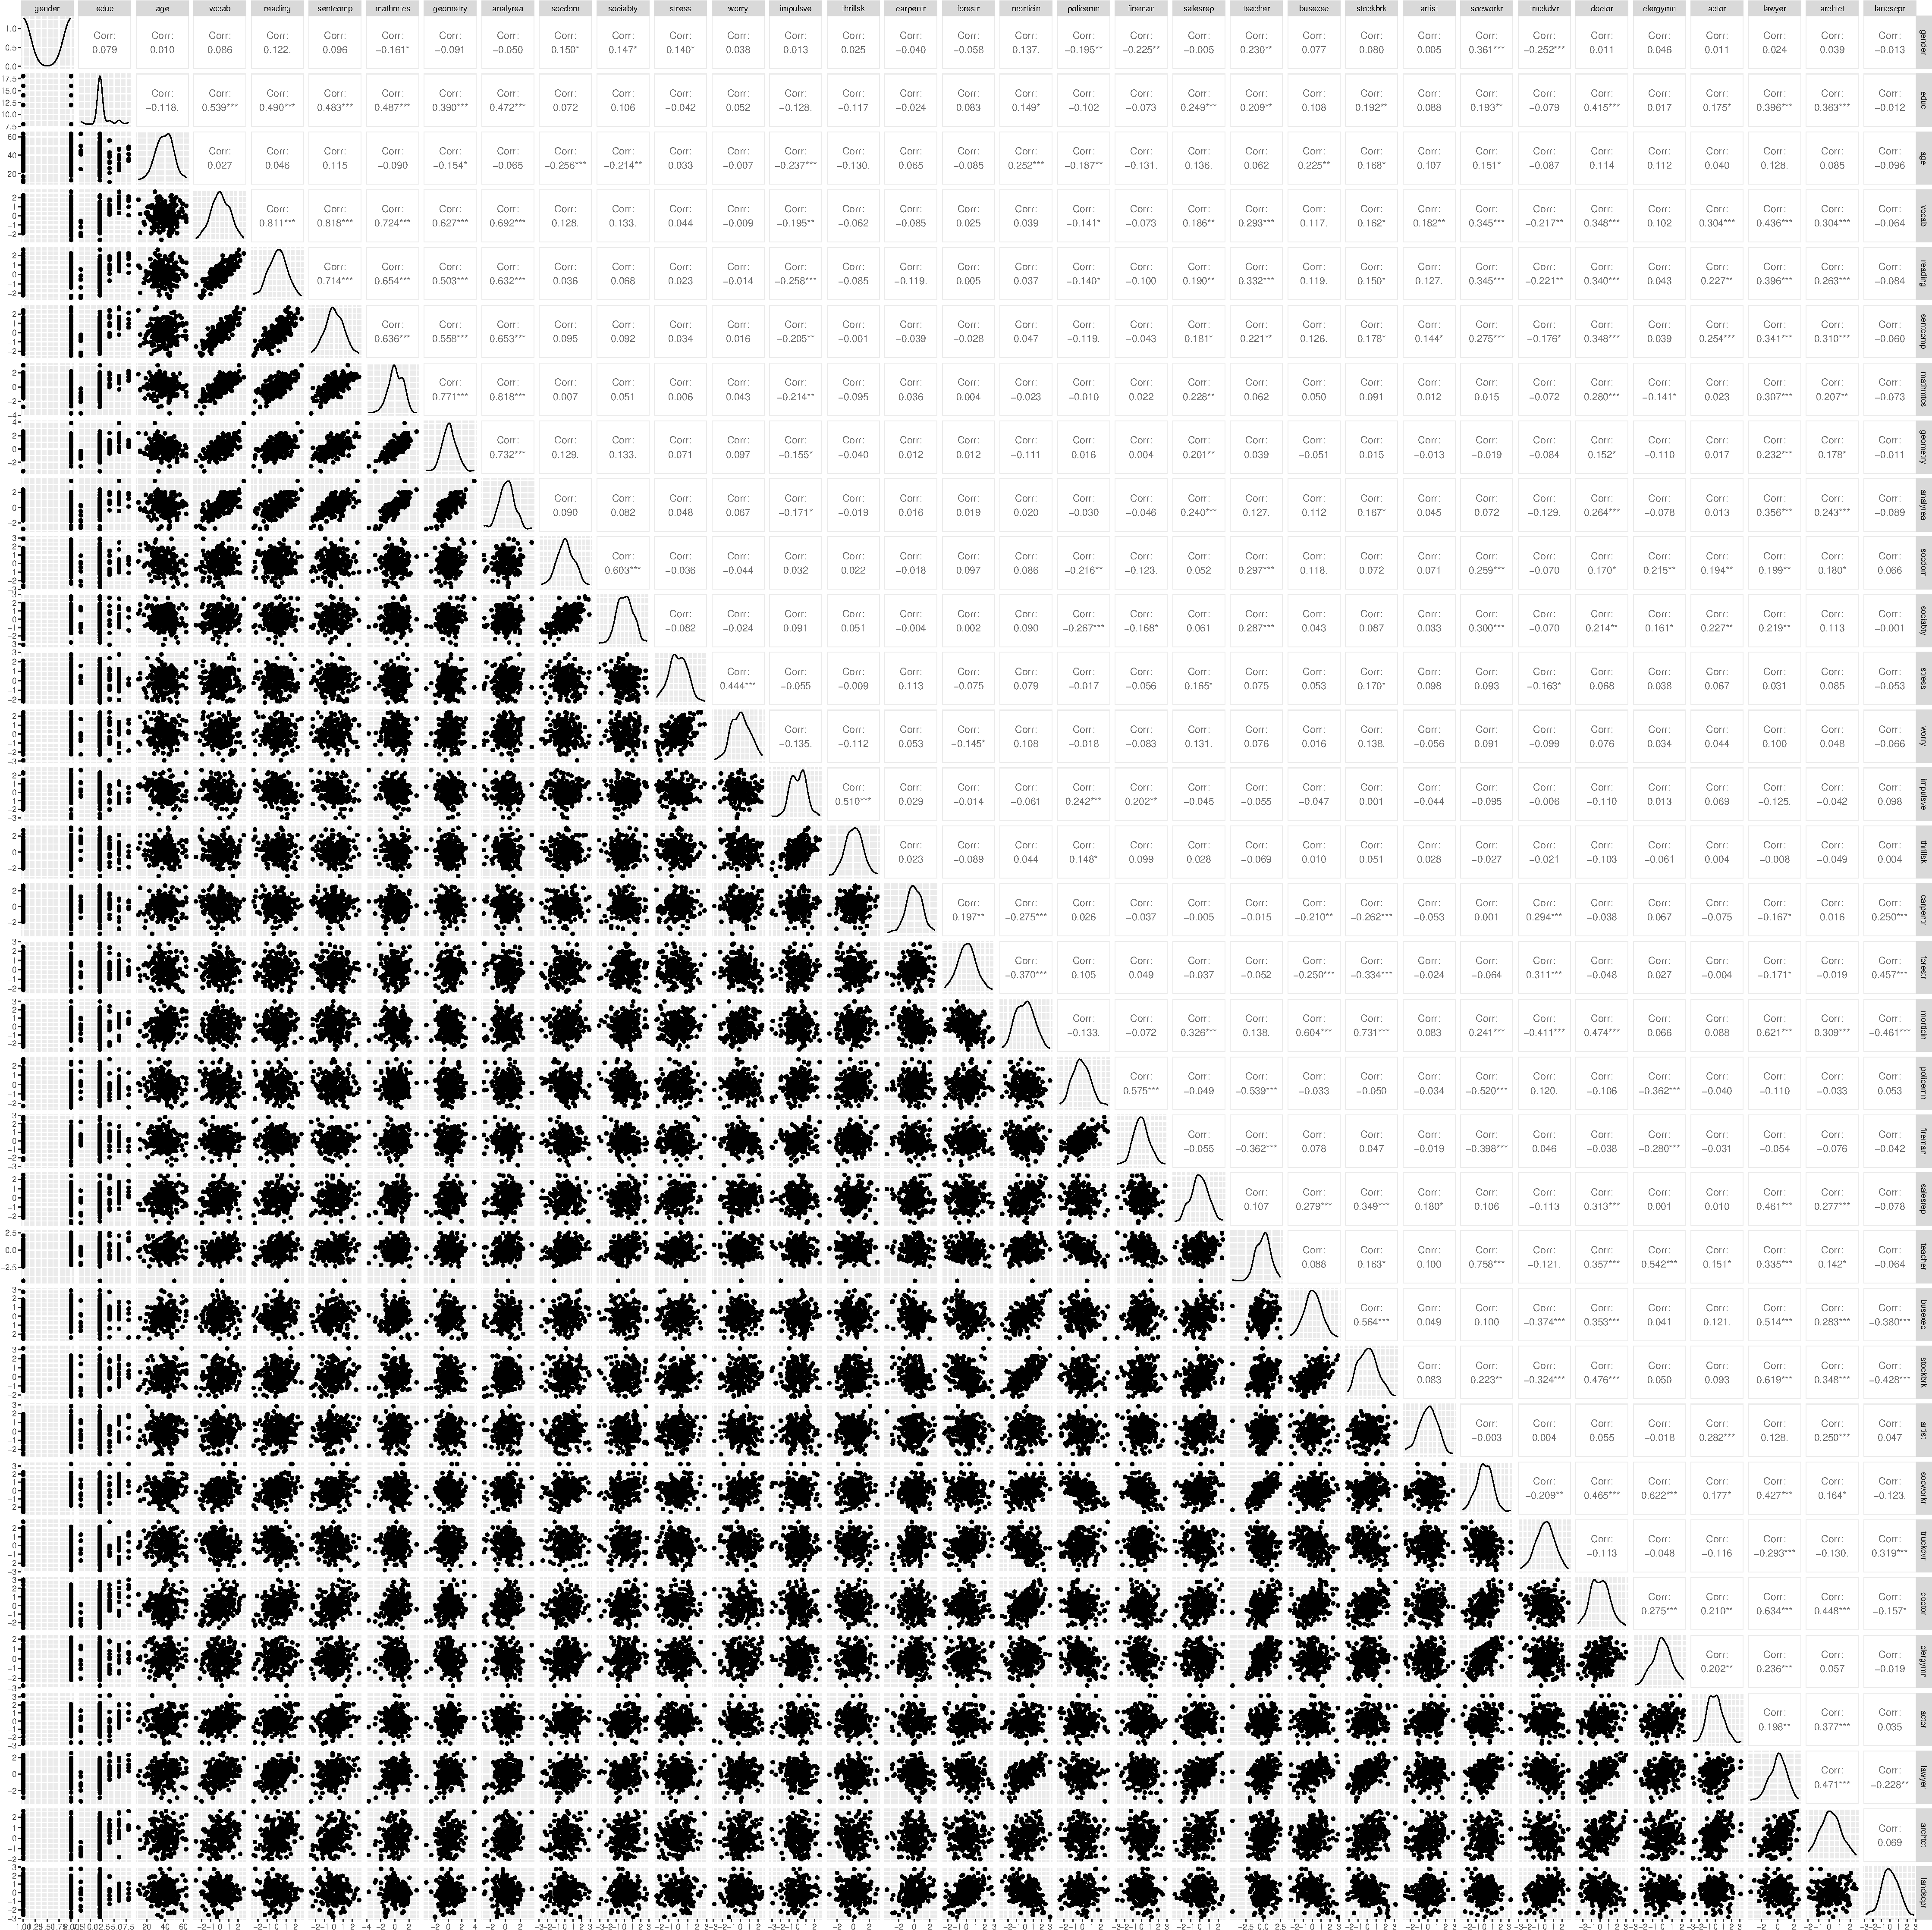
\includegraphics{Project_files/figure-latex/unnamed-chunk-5-1.pdf}

The highest prices in europe are found in amsterdam.

\hypertarget{density-plot-of-price-vs-room-type}{%
\subsubsection{Density plot of Price vs Room
type}\label{density-plot-of-price-vs-room-type}}

\begin{Shaded}
\begin{Highlighting}[]
\FunctionTok{ggplot}\NormalTok{(my\_data\_filtered, }\FunctionTok{aes}\NormalTok{(}\AttributeTok{x =}\NormalTok{ realSum, }\AttributeTok{group =}\NormalTok{ room\_type,}
    \AttributeTok{fill =}\NormalTok{ room\_type, }\AttributeTok{alpha =} \FloatTok{0.2}\NormalTok{)) }\SpecialCharTok{+} \FunctionTok{geom\_density}\NormalTok{()}
\end{Highlighting}
\end{Shaded}

\includegraphics{Project_files/figure-latex/unnamed-chunk-6-1.pdf}

The prices of entire home are high comparitively

\hypertarget{boxplot-of-city-vs-guest-satisfaction}{%
\subsubsection{Boxplot of City vs Guest
Satisfaction}\label{boxplot-of-city-vs-guest-satisfaction}}

\begin{Shaded}
\begin{Highlighting}[]
\FunctionTok{ggplot}\NormalTok{(my\_data\_filtered, }\FunctionTok{aes}\NormalTok{(}\AttributeTok{x =} \FunctionTok{reorder}\NormalTok{(city\_day, guest\_satisfaction\_overall,}
    \AttributeTok{FUN =}\NormalTok{ median), }\AttributeTok{y =}\NormalTok{ guest\_satisfaction\_overall, }\AttributeTok{fill =}\NormalTok{ city\_day)) }\SpecialCharTok{+}
    \FunctionTok{geom\_boxplot}\NormalTok{() }\SpecialCharTok{+} \FunctionTok{coord\_flip}\NormalTok{() }\SpecialCharTok{+} \FunctionTok{theme}\NormalTok{(}\AttributeTok{legend.key.height =} \FunctionTok{unit}\NormalTok{(}\FloatTok{0.5}\NormalTok{,}
    \StringTok{"cm"}\NormalTok{), }\AttributeTok{legend.key.size =} \FunctionTok{unit}\NormalTok{(}\DecValTok{1}\NormalTok{, }\StringTok{"lines"}\NormalTok{))}
\end{Highlighting}
\end{Shaded}

\includegraphics{Project_files/figure-latex/unnamed-chunk-7-1.pdf}

This plot shows there is no major difference in Guest Satisfaction vs
City.

\hypertarget{scatterplot-of-price-vs-guest-satisfaction-filtered-by-city}{%
\subsubsection{Scatterplot of Price vs Guest Satisfaction filtered by
city}\label{scatterplot-of-price-vs-guest-satisfaction-filtered-by-city}}

\begin{Shaded}
\begin{Highlighting}[]
\FunctionTok{ggplot}\NormalTok{(my\_data\_filtered, }\FunctionTok{aes}\NormalTok{(}\AttributeTok{x =}\NormalTok{ realSum, }\AttributeTok{y =}\NormalTok{ guest\_satisfaction\_overall,}
    \AttributeTok{color =}\NormalTok{ city\_day)) }\SpecialCharTok{+} \FunctionTok{geom\_point}\NormalTok{() }\SpecialCharTok{+} \FunctionTok{xlab}\NormalTok{(}\StringTok{"Price"}\NormalTok{) }\SpecialCharTok{+} \FunctionTok{ylab}\NormalTok{(}\StringTok{"Guest Satisfaction Overall"}\NormalTok{) }\SpecialCharTok{+}
    \FunctionTok{scale\_color\_discrete}\NormalTok{(}\AttributeTok{name =} \StringTok{"City{-}Day"}\NormalTok{)}
\end{Highlighting}
\end{Shaded}

\includegraphics{Project_files/figure-latex/unnamed-chunk-8-1.pdf}

This plot implies there are good cheaper Airbnb at most cities which
give higher guest satisfaction rating

\hypertarget{scatterplot-of-prices-in-rome-w.r.t-latitude-and-longitude-during-weekdays}{%
\subsubsection{Scatterplot of Prices in Rome w.r.t Latitude and
Longitude during
weekdays}\label{scatterplot-of-prices-in-rome-w.r.t-latitude-and-longitude-during-weekdays}}

\begin{Shaded}
\begin{Highlighting}[]
\NormalTok{tema }\OtherTok{\textless{}{-}} \FunctionTok{theme}\NormalTok{(}\AttributeTok{plot.title =} \FunctionTok{element\_text}\NormalTok{(}\AttributeTok{size =} \DecValTok{23}\NormalTok{, }\AttributeTok{hjust =} \FloatTok{0.5}\NormalTok{),}
    \AttributeTok{axis.text.x =} \FunctionTok{element\_text}\NormalTok{(}\AttributeTok{size =} \DecValTok{19}\NormalTok{, }\AttributeTok{face =} \StringTok{"bold"}\NormalTok{), }\AttributeTok{axis.text.y =} \FunctionTok{element\_text}\NormalTok{(}\AttributeTok{size =} \DecValTok{19}\NormalTok{,}
        \AttributeTok{face =} \StringTok{"bold"}\NormalTok{), }\AttributeTok{axis.title.x =} \FunctionTok{element\_text}\NormalTok{(}\AttributeTok{size =} \DecValTok{19}\NormalTok{),}
    \AttributeTok{axis.title.y =} \FunctionTok{element\_text}\NormalTok{(}\AttributeTok{size =} \DecValTok{19}\NormalTok{), }\AttributeTok{legend.text =} \FunctionTok{element\_text}\NormalTok{(}\AttributeTok{colour =} \StringTok{"black"}\NormalTok{,}
        \AttributeTok{size =} \DecValTok{19}\NormalTok{, }\AttributeTok{face =} \StringTok{"bold"}\NormalTok{), }\AttributeTok{legend.background =} \FunctionTok{element\_rect}\NormalTok{(}\AttributeTok{fill =} \StringTok{"\#F5FFFA"}\NormalTok{,}
        \AttributeTok{size =} \FloatTok{0.5}\NormalTok{, }\AttributeTok{linetype =} \StringTok{"dashed"}\NormalTok{, }\AttributeTok{colour =} \StringTok{"black"}\NormalTok{))}

\NormalTok{rome\_data }\OtherTok{\textless{}{-}}\NormalTok{ my\_data\_filtered }\SpecialCharTok{\%\textgreater{}\%}
    \FunctionTok{subset}\NormalTok{(city\_day }\SpecialCharTok{==} \StringTok{"rome\_weekdays"}\NormalTok{)}

\FunctionTok{ggplot}\NormalTok{(}\AttributeTok{data =}\NormalTok{ rome\_data, }\AttributeTok{mapping =} \FunctionTok{aes}\NormalTok{(}\AttributeTok{x =}\NormalTok{ lat, }\AttributeTok{y =}\NormalTok{ lng)) }\SpecialCharTok{+} \FunctionTok{theme\_minimal}\NormalTok{() }\SpecialCharTok{+}
    \FunctionTok{scale\_fill\_identity}\NormalTok{() }\SpecialCharTok{+} \FunctionTok{geom\_point}\NormalTok{(}\AttributeTok{mapping =} \FunctionTok{aes}\NormalTok{(}\AttributeTok{color =}\NormalTok{ realSum),}
    \AttributeTok{size =} \DecValTok{3}\NormalTok{) }\SpecialCharTok{+} \FunctionTok{ggtitle}\NormalTok{(}\StringTok{""}\NormalTok{) }\SpecialCharTok{+}\NormalTok{ tema}
\end{Highlighting}
\end{Shaded}

\includegraphics{Project_files/figure-latex/unnamed-chunk-9-1.pdf}

This plot is within expectations of game theory, which suggests similar
types of establishments (price and hospitality) tend be in clusters.

\hypertarget{outlier-analysis}{%
\subsubsection{Outlier Analysis}\label{outlier-analysis}}

\begin{Shaded}
\begin{Highlighting}[]
\FunctionTok{ggplot}\NormalTok{(my\_outliers, }\FunctionTok{aes}\NormalTok{(}\AttributeTok{x =}\NormalTok{ realSum, }\AttributeTok{y =}\NormalTok{ dist)) }\SpecialCharTok{+} \FunctionTok{geom\_point}\NormalTok{(}\AttributeTok{alpha =} \FloatTok{0.5}\NormalTok{) }\SpecialCharTok{+}
    \FunctionTok{theme}\NormalTok{(}\AttributeTok{axis.title.x =} \FunctionTok{element\_text}\NormalTok{(}\AttributeTok{size =} \DecValTok{14}\NormalTok{), }\AttributeTok{axis.title.y =} \FunctionTok{element\_text}\NormalTok{(}\AttributeTok{size =} \DecValTok{14}\NormalTok{))}
\end{Highlighting}
\end{Shaded}

\includegraphics{Project_files/figure-latex/unnamed-chunk-10-1.pdf}

\begin{Shaded}
\begin{Highlighting}[]
\FunctionTok{ggplot}\NormalTok{(my\_outliers, }\FunctionTok{aes}\NormalTok{(}\AttributeTok{x =}\NormalTok{ realSum, }\AttributeTok{fill =}\NormalTok{ cleanliness\_rating,}
    \AttributeTok{group =}\NormalTok{ cleanliness\_rating)) }\SpecialCharTok{+} \FunctionTok{geom\_density}\NormalTok{(}\AttributeTok{alpha =} \FloatTok{0.5}\NormalTok{) }\SpecialCharTok{+}
    \FunctionTok{theme}\NormalTok{(}\AttributeTok{axis.title.x =} \FunctionTok{element\_text}\NormalTok{(}\AttributeTok{size =} \DecValTok{14}\NormalTok{), }\AttributeTok{axis.title.y =} \FunctionTok{element\_text}\NormalTok{(}\AttributeTok{size =} \DecValTok{14}\NormalTok{)) }\SpecialCharTok{+}
    \FunctionTok{facet\_wrap}\NormalTok{(}\SpecialCharTok{\textasciitilde{}}\NormalTok{cleanliness\_rating)}
\end{Highlighting}
\end{Shaded}

\includegraphics{Project_files/figure-latex/unnamed-chunk-11-1.pdf}

\begin{Shaded}
\begin{Highlighting}[]
\FunctionTok{ggplot}\NormalTok{(my\_outliers, }\FunctionTok{aes}\NormalTok{(}\AttributeTok{x =}\NormalTok{ realSum, }\AttributeTok{fill =}\NormalTok{ room\_shared, }\AttributeTok{group =}\NormalTok{ room\_shared)) }\SpecialCharTok{+}
    \FunctionTok{geom\_density}\NormalTok{(}\AttributeTok{alpha =} \FloatTok{0.5}\NormalTok{) }\SpecialCharTok{+} \FunctionTok{theme}\NormalTok{(}\AttributeTok{axis.title.x =} \FunctionTok{element\_text}\NormalTok{(}\AttributeTok{size =} \DecValTok{14}\NormalTok{),}
    \AttributeTok{axis.title.y =} \FunctionTok{element\_text}\NormalTok{(}\AttributeTok{size =} \DecValTok{14}\NormalTok{))}
\end{Highlighting}
\end{Shaded}

\includegraphics{Project_files/figure-latex/unnamed-chunk-12-1.pdf}

\begin{Shaded}
\begin{Highlighting}[]
\FunctionTok{ggplot}\NormalTok{(my\_outliers, }\FunctionTok{aes}\NormalTok{(}\AttributeTok{x =}\NormalTok{ realSum, }\AttributeTok{fill =}\NormalTok{ room\_private, }\AttributeTok{group =}\NormalTok{ room\_private)) }\SpecialCharTok{+}
    \FunctionTok{geom\_histogram}\NormalTok{(}\AttributeTok{alpha =} \FloatTok{0.5}\NormalTok{, }\AttributeTok{bins =} \DecValTok{20}\NormalTok{) }\SpecialCharTok{+} \FunctionTok{theme}\NormalTok{(}\AttributeTok{axis.title.x =} \FunctionTok{element\_text}\NormalTok{(}\AttributeTok{size =} \DecValTok{14}\NormalTok{),}
    \AttributeTok{axis.title.y =} \FunctionTok{element\_text}\NormalTok{(}\AttributeTok{size =} \DecValTok{14}\NormalTok{))}
\end{Highlighting}
\end{Shaded}

\includegraphics{Project_files/figure-latex/unnamed-chunk-13-1.pdf}

\begin{Shaded}
\begin{Highlighting}[]
\FunctionTok{ggplot}\NormalTok{(my\_outliers, }\FunctionTok{aes}\NormalTok{(}\AttributeTok{x =}\NormalTok{ realSum, }\AttributeTok{fill =}\NormalTok{ multi, }\AttributeTok{group =}\NormalTok{ multi)) }\SpecialCharTok{+}
    \FunctionTok{geom\_histogram}\NormalTok{(}\AttributeTok{alpha =} \FloatTok{0.5}\NormalTok{, }\AttributeTok{bins =} \DecValTok{20}\NormalTok{) }\SpecialCharTok{+} \FunctionTok{theme}\NormalTok{(}\AttributeTok{axis.title.x =} \FunctionTok{element\_text}\NormalTok{(}\AttributeTok{size =} \DecValTok{14}\NormalTok{),}
    \AttributeTok{axis.title.y =} \FunctionTok{element\_text}\NormalTok{(}\AttributeTok{size =} \DecValTok{14}\NormalTok{))}
\end{Highlighting}
\end{Shaded}

\includegraphics{Project_files/figure-latex/unnamed-chunk-14-1.pdf}

\begin{Shaded}
\begin{Highlighting}[]
\FunctionTok{ggplot}\NormalTok{() }\SpecialCharTok{+} \FunctionTok{geom\_point}\NormalTok{(}\AttributeTok{data =}\NormalTok{ my\_data\_filtered, }\FunctionTok{aes}\NormalTok{(}\AttributeTok{x =}\NormalTok{ realSum,}
    \AttributeTok{y =}\NormalTok{ metro\_dist, }\AttributeTok{color =} \StringTok{"Filtered Data"}\NormalTok{), }\AttributeTok{alpha =} \FloatTok{0.4}\NormalTok{) }\SpecialCharTok{+}
    \FunctionTok{geom\_point}\NormalTok{(}\AttributeTok{data =}\NormalTok{ my\_outliers, }\FunctionTok{aes}\NormalTok{(}\AttributeTok{x =}\NormalTok{ realSum, }\AttributeTok{y =}\NormalTok{ metro\_dist,}
        \AttributeTok{color =} \StringTok{"Outliers"}\NormalTok{), }\AttributeTok{alpha =} \FloatTok{0.4}\NormalTok{) }\SpecialCharTok{+} \FunctionTok{scale\_color\_manual}\NormalTok{(}\AttributeTok{values =} \FunctionTok{c}\NormalTok{(}\StringTok{\textasciigrave{}}\AttributeTok{Filtered Data}\StringTok{\textasciigrave{}} \OtherTok{=} \StringTok{"blue"}\NormalTok{,}
    \AttributeTok{Outliers =} \StringTok{"red"}\NormalTok{))}
\end{Highlighting}
\end{Shaded}

\includegraphics{Project_files/figure-latex/unnamed-chunk-15-1.pdf}

\begin{Shaded}
\begin{Highlighting}[]
\FunctionTok{ggplot}\NormalTok{() }\SpecialCharTok{+} \FunctionTok{geom\_point}\NormalTok{(}\AttributeTok{data =}\NormalTok{ my\_data\_filtered, }\FunctionTok{aes}\NormalTok{(}\AttributeTok{x =}\NormalTok{ realSum,}
    \AttributeTok{y =}\NormalTok{ metro\_dist, }\AttributeTok{color =} \StringTok{"Filtered Data"}\NormalTok{), }\AttributeTok{alpha =} \FloatTok{0.4}\NormalTok{) }\SpecialCharTok{+}
    \FunctionTok{geom\_point}\NormalTok{(}\AttributeTok{data =}\NormalTok{ my\_outliers, }\FunctionTok{aes}\NormalTok{(}\AttributeTok{x =}\NormalTok{ realSum, }\AttributeTok{y =}\NormalTok{ metro\_dist,}
        \AttributeTok{color =} \StringTok{"Outliers"}\NormalTok{), }\AttributeTok{alpha =} \FloatTok{0.4}\NormalTok{) }\SpecialCharTok{+} \FunctionTok{scale\_color\_manual}\NormalTok{(}\AttributeTok{values =} \FunctionTok{c}\NormalTok{(}\StringTok{\textasciigrave{}}\AttributeTok{Filtered Data}\StringTok{\textasciigrave{}} \OtherTok{=} \StringTok{"blue"}\NormalTok{,}
    \AttributeTok{Outliers =} \StringTok{"red"}\NormalTok{)) }\SpecialCharTok{+} \FunctionTok{facet\_wrap}\NormalTok{(}\SpecialCharTok{\textasciitilde{}}\NormalTok{city\_day)}
\end{Highlighting}
\end{Shaded}

\includegraphics{Project_files/figure-latex/unnamed-chunk-15-2.pdf}

The pricey rooms are mostly near to the metro

\begin{Shaded}
\begin{Highlighting}[]
\FunctionTok{ggplot}\NormalTok{() }\SpecialCharTok{+} \FunctionTok{geom\_point}\NormalTok{(}\AttributeTok{data =}\NormalTok{ my\_data\_filtered, }\FunctionTok{aes}\NormalTok{(}\AttributeTok{x =}\NormalTok{ realSum,}
    \AttributeTok{y =}\NormalTok{ dist, }\AttributeTok{color =} \StringTok{"Filtered Data"}\NormalTok{), }\AttributeTok{alpha =} \FloatTok{0.4}\NormalTok{) }\SpecialCharTok{+} \FunctionTok{geom\_point}\NormalTok{(}\AttributeTok{data =}\NormalTok{ my\_outliers,}
    \FunctionTok{aes}\NormalTok{(}\AttributeTok{x =}\NormalTok{ realSum, }\AttributeTok{y =}\NormalTok{ dist, }\AttributeTok{color =} \StringTok{"Outliers"}\NormalTok{), }\AttributeTok{alpha =} \FloatTok{0.4}\NormalTok{) }\SpecialCharTok{+}
    \FunctionTok{scale\_color\_manual}\NormalTok{(}\AttributeTok{values =} \FunctionTok{c}\NormalTok{(}\StringTok{\textasciigrave{}}\AttributeTok{Filtered Data}\StringTok{\textasciigrave{}} \OtherTok{=} \StringTok{"blue"}\NormalTok{, }\AttributeTok{Outliers =} \StringTok{"red"}\NormalTok{))}
\end{Highlighting}
\end{Shaded}

\includegraphics{Project_files/figure-latex/unnamed-chunk-16-1.pdf}

\begin{Shaded}
\begin{Highlighting}[]
\FunctionTok{ggplot}\NormalTok{() }\SpecialCharTok{+} \FunctionTok{geom\_point}\NormalTok{(}\AttributeTok{data =}\NormalTok{ my\_data\_filtered, }\FunctionTok{aes}\NormalTok{(}\AttributeTok{x =}\NormalTok{ realSum,}
    \AttributeTok{y =}\NormalTok{ dist, }\AttributeTok{color =} \StringTok{"Filtered Data"}\NormalTok{), }\AttributeTok{alpha =} \FloatTok{0.4}\NormalTok{) }\SpecialCharTok{+} \FunctionTok{geom\_point}\NormalTok{(}\AttributeTok{data =}\NormalTok{ my\_outliers,}
    \FunctionTok{aes}\NormalTok{(}\AttributeTok{x =}\NormalTok{ realSum, }\AttributeTok{y =}\NormalTok{ dist, }\AttributeTok{color =} \StringTok{"Outliers"}\NormalTok{), }\AttributeTok{alpha =} \FloatTok{0.4}\NormalTok{) }\SpecialCharTok{+}
    \FunctionTok{scale\_color\_manual}\NormalTok{(}\AttributeTok{values =} \FunctionTok{c}\NormalTok{(}\StringTok{\textasciigrave{}}\AttributeTok{Filtered Data}\StringTok{\textasciigrave{}} \OtherTok{=} \StringTok{"blue"}\NormalTok{, }\AttributeTok{Outliers =} \StringTok{"red"}\NormalTok{)) }\SpecialCharTok{+}
    \FunctionTok{facet\_wrap}\NormalTok{(}\SpecialCharTok{\textasciitilde{}}\NormalTok{city\_day)}
\end{Highlighting}
\end{Shaded}

\includegraphics{Project_files/figure-latex/unnamed-chunk-16-2.pdf}

The pricey rooms are mostly near to the centre of the city and the there
is some correlation.

\begin{Shaded}
\begin{Highlighting}[]
\FunctionTok{ggplot}\NormalTok{() }\SpecialCharTok{+} \FunctionTok{geom\_point}\NormalTok{(}\AttributeTok{data =}\NormalTok{ my\_data\_filtered, }\FunctionTok{aes}\NormalTok{(}\AttributeTok{x =}\NormalTok{ realSum,}
    \AttributeTok{y =}\NormalTok{ attr\_index, }\AttributeTok{color =} \StringTok{"Filtered Data"}\NormalTok{), }\AttributeTok{alpha =} \FloatTok{0.4}\NormalTok{) }\SpecialCharTok{+}
    \FunctionTok{geom\_point}\NormalTok{(}\AttributeTok{data =}\NormalTok{ my\_outliers, }\FunctionTok{aes}\NormalTok{(}\AttributeTok{x =}\NormalTok{ realSum, }\AttributeTok{y =}\NormalTok{ attr\_index,}
        \AttributeTok{color =} \StringTok{"Outliers"}\NormalTok{), }\AttributeTok{alpha =} \FloatTok{0.4}\NormalTok{) }\SpecialCharTok{+} \FunctionTok{scale\_color\_manual}\NormalTok{(}\AttributeTok{values =} \FunctionTok{c}\NormalTok{(}\StringTok{\textasciigrave{}}\AttributeTok{Filtered Data}\StringTok{\textasciigrave{}} \OtherTok{=} \StringTok{"blue"}\NormalTok{,}
    \AttributeTok{Outliers =} \StringTok{"red"}\NormalTok{))}
\end{Highlighting}
\end{Shaded}

\includegraphics{Project_files/figure-latex/unnamed-chunk-17-1.pdf}

\begin{Shaded}
\begin{Highlighting}[]
\FunctionTok{ggplot}\NormalTok{() }\SpecialCharTok{+} \FunctionTok{geom\_point}\NormalTok{(}\AttributeTok{data =}\NormalTok{ my\_data\_filtered, }\FunctionTok{aes}\NormalTok{(}\AttributeTok{x =}\NormalTok{ realSum,}
    \AttributeTok{y =}\NormalTok{ attr\_index, }\AttributeTok{color =} \StringTok{"Filtered Data"}\NormalTok{), }\AttributeTok{alpha =} \FloatTok{0.4}\NormalTok{) }\SpecialCharTok{+}
    \FunctionTok{geom\_point}\NormalTok{(}\AttributeTok{data =}\NormalTok{ my\_outliers, }\FunctionTok{aes}\NormalTok{(}\AttributeTok{x =}\NormalTok{ realSum, }\AttributeTok{y =}\NormalTok{ attr\_index,}
        \AttributeTok{color =} \StringTok{"Outliers"}\NormalTok{), }\AttributeTok{alpha =} \FloatTok{0.4}\NormalTok{) }\SpecialCharTok{+} \FunctionTok{scale\_color\_manual}\NormalTok{(}\AttributeTok{values =} \FunctionTok{c}\NormalTok{(}\StringTok{\textasciigrave{}}\AttributeTok{Filtered Data}\StringTok{\textasciigrave{}} \OtherTok{=} \StringTok{"blue"}\NormalTok{,}
    \AttributeTok{Outliers =} \StringTok{"red"}\NormalTok{)) }\SpecialCharTok{+} \FunctionTok{facet\_wrap}\NormalTok{(}\SpecialCharTok{\textasciitilde{}}\NormalTok{city\_day)}
\end{Highlighting}
\end{Shaded}

\includegraphics{Project_files/figure-latex/unnamed-chunk-17-2.pdf}

The range of values falling b/w outliers and normal data is almost same
. So there isn't a relationship b/w attr\_index and realSum.

\begin{Shaded}
\begin{Highlighting}[]
\FunctionTok{ggplot}\NormalTok{() }\SpecialCharTok{+} \FunctionTok{geom\_point}\NormalTok{(}\AttributeTok{data =}\NormalTok{ my\_data, }\FunctionTok{aes}\NormalTok{(}\AttributeTok{x =}\NormalTok{ attr\_index, }\AttributeTok{y =}\NormalTok{ attr\_index\_norm,}
    \AttributeTok{color =} \StringTok{"Filtered Data"}\NormalTok{), }\AttributeTok{alpha =} \FloatTok{0.4}\NormalTok{) }\SpecialCharTok{+} \FunctionTok{scale\_color\_manual}\NormalTok{(}\AttributeTok{values =} \FunctionTok{c}\NormalTok{(}\StringTok{\textasciigrave{}}\AttributeTok{Filtered Data}\StringTok{\textasciigrave{}} \OtherTok{=} \StringTok{"blue"}\NormalTok{,}
    \AttributeTok{Outliers =} \StringTok{"red"}\NormalTok{))}
\end{Highlighting}
\end{Shaded}

\includegraphics{Project_files/figure-latex/unnamed-chunk-18-1.pdf}

\begin{Shaded}
\begin{Highlighting}[]
\FunctionTok{ggplot}\NormalTok{() }\SpecialCharTok{+} \FunctionTok{geom\_point}\NormalTok{(}\AttributeTok{data =}\NormalTok{ my\_data, }\FunctionTok{aes}\NormalTok{(}\AttributeTok{x =}\NormalTok{ attr\_index, }\AttributeTok{y =}\NormalTok{ attr\_index\_norm,}
    \AttributeTok{color =} \StringTok{"Filtered Data"}\NormalTok{), }\AttributeTok{alpha =} \FloatTok{0.4}\NormalTok{) }\SpecialCharTok{+} \FunctionTok{scale\_color\_manual}\NormalTok{(}\AttributeTok{values =} \FunctionTok{c}\NormalTok{(}\StringTok{\textasciigrave{}}\AttributeTok{Filtered Data}\StringTok{\textasciigrave{}} \OtherTok{=} \StringTok{"blue"}\NormalTok{,}
    \AttributeTok{Outliers =} \StringTok{"red"}\NormalTok{)) }\SpecialCharTok{+} \FunctionTok{facet\_wrap}\NormalTok{(}\SpecialCharTok{\textasciitilde{}}\NormalTok{city\_day)}
\end{Highlighting}
\end{Shaded}

\includegraphics{Project_files/figure-latex/unnamed-chunk-18-2.pdf}

attr\_index and attr\_index\_norm are same, attr\_index\_norm is just
normalized attr\_index

\begin{Shaded}
\begin{Highlighting}[]
\FunctionTok{ggplot}\NormalTok{() }\SpecialCharTok{+} \FunctionTok{geom\_point}\NormalTok{(}\AttributeTok{data =}\NormalTok{ my\_data, }\FunctionTok{aes}\NormalTok{(}\AttributeTok{x =}\NormalTok{ rest\_index, }\AttributeTok{y =}\NormalTok{ rest\_index\_norm,}
    \AttributeTok{color =} \StringTok{"Filtered Data"}\NormalTok{), }\AttributeTok{alpha =} \FloatTok{0.4}\NormalTok{) }\SpecialCharTok{+} \FunctionTok{scale\_color\_manual}\NormalTok{(}\AttributeTok{values =} \FunctionTok{c}\NormalTok{(}\StringTok{\textasciigrave{}}\AttributeTok{Filtered Data}\StringTok{\textasciigrave{}} \OtherTok{=} \StringTok{"blue"}\NormalTok{,}
    \AttributeTok{Outliers =} \StringTok{"red"}\NormalTok{))}
\end{Highlighting}
\end{Shaded}

\includegraphics{Project_files/figure-latex/unnamed-chunk-19-1.pdf}

\begin{Shaded}
\begin{Highlighting}[]
\FunctionTok{ggplot}\NormalTok{() }\SpecialCharTok{+} \FunctionTok{geom\_point}\NormalTok{(}\AttributeTok{data =}\NormalTok{ my\_data, }\FunctionTok{aes}\NormalTok{(}\AttributeTok{x =}\NormalTok{ rest\_index, }\AttributeTok{y =}\NormalTok{ rest\_index\_norm,}
    \AttributeTok{color =} \StringTok{"Filtered Data"}\NormalTok{), }\AttributeTok{alpha =} \FloatTok{0.4}\NormalTok{) }\SpecialCharTok{+} \FunctionTok{scale\_color\_manual}\NormalTok{(}\AttributeTok{values =} \FunctionTok{c}\NormalTok{(}\StringTok{\textasciigrave{}}\AttributeTok{Filtered Data}\StringTok{\textasciigrave{}} \OtherTok{=} \StringTok{"blue"}\NormalTok{,}
    \AttributeTok{Outliers =} \StringTok{"red"}\NormalTok{)) }\SpecialCharTok{+} \FunctionTok{facet\_wrap}\NormalTok{(}\SpecialCharTok{\textasciitilde{}}\NormalTok{city\_day)}
\end{Highlighting}
\end{Shaded}

\includegraphics{Project_files/figure-latex/unnamed-chunk-19-2.pdf}

rest\_index and rest\_index\_norm are same, rest\_index\_norm is just
normalized rest\_index

\begin{Shaded}
\begin{Highlighting}[]
\FunctionTok{ggplot}\NormalTok{() }\SpecialCharTok{+} \FunctionTok{geom\_point}\NormalTok{(}\AttributeTok{data =}\NormalTok{ my\_data\_filtered, }\FunctionTok{aes}\NormalTok{(}\AttributeTok{x =}\NormalTok{ realSum,}
    \AttributeTok{y =}\NormalTok{ rest\_index, }\AttributeTok{color =} \StringTok{"Filtered Data"}\NormalTok{), }\AttributeTok{alpha =} \FloatTok{0.4}\NormalTok{) }\SpecialCharTok{+}
    \FunctionTok{geom\_point}\NormalTok{(}\AttributeTok{data =}\NormalTok{ my\_outliers, }\FunctionTok{aes}\NormalTok{(}\AttributeTok{x =}\NormalTok{ realSum, }\AttributeTok{y =}\NormalTok{ rest\_index,}
        \AttributeTok{color =} \StringTok{"Outliers"}\NormalTok{), }\AttributeTok{alpha =} \FloatTok{0.4}\NormalTok{) }\SpecialCharTok{+} \FunctionTok{scale\_color\_manual}\NormalTok{(}\AttributeTok{values =} \FunctionTok{c}\NormalTok{(}\StringTok{\textasciigrave{}}\AttributeTok{Filtered Data}\StringTok{\textasciigrave{}} \OtherTok{=} \StringTok{"blue"}\NormalTok{,}
    \AttributeTok{Outliers =} \StringTok{"red"}\NormalTok{))}
\end{Highlighting}
\end{Shaded}

\includegraphics{Project_files/figure-latex/unnamed-chunk-20-1.pdf}

\begin{Shaded}
\begin{Highlighting}[]
\FunctionTok{ggplot}\NormalTok{() }\SpecialCharTok{+} \FunctionTok{geom\_point}\NormalTok{(}\AttributeTok{data =}\NormalTok{ my\_data\_filtered, }\FunctionTok{aes}\NormalTok{(}\AttributeTok{x =}\NormalTok{ realSum,}
    \AttributeTok{y =}\NormalTok{ rest\_index, }\AttributeTok{color =} \StringTok{"Filtered Data"}\NormalTok{), }\AttributeTok{alpha =} \FloatTok{0.4}\NormalTok{) }\SpecialCharTok{+}
    \FunctionTok{geom\_point}\NormalTok{(}\AttributeTok{data =}\NormalTok{ my\_outliers, }\FunctionTok{aes}\NormalTok{(}\AttributeTok{x =}\NormalTok{ realSum, }\AttributeTok{y =}\NormalTok{ rest\_index,}
        \AttributeTok{color =} \StringTok{"Outliers"}\NormalTok{), }\AttributeTok{alpha =} \FloatTok{0.4}\NormalTok{) }\SpecialCharTok{+} \FunctionTok{scale\_color\_manual}\NormalTok{(}\AttributeTok{values =} \FunctionTok{c}\NormalTok{(}\StringTok{\textasciigrave{}}\AttributeTok{Filtered Data}\StringTok{\textasciigrave{}} \OtherTok{=} \StringTok{"blue"}\NormalTok{,}
    \AttributeTok{Outliers =} \StringTok{"red"}\NormalTok{)) }\SpecialCharTok{+} \FunctionTok{facet\_wrap}\NormalTok{(}\SpecialCharTok{\textasciitilde{}}\NormalTok{city\_day)}
\end{Highlighting}
\end{Shaded}

\includegraphics{Project_files/figure-latex/unnamed-chunk-20-2.pdf}

There is no relationship outliers and rest\_index

\hypertarget{percentage-of-outliers.}{%
\subsubsection{Percentage of Outliers.}\label{percentage-of-outliers.}}

\begin{Shaded}
\begin{Highlighting}[]
\CommentTok{\# Create empty table}
\NormalTok{outliers\_table }\OtherTok{\textless{}{-}} \FunctionTok{data.frame}\NormalTok{(}\AttributeTok{City\_day =} \FunctionTok{character}\NormalTok{(), }\AttributeTok{Data\_Length =} \FunctionTok{numeric}\NormalTok{(),}
    \AttributeTok{Percent\_Outliers =} \FunctionTok{numeric}\NormalTok{(), }\AttributeTok{stringsAsFactors =} \ConstantTok{FALSE}\NormalTok{)}

\CommentTok{\# Loop through city\_data and fill in table}
\ControlFlowTok{for}\NormalTok{ (city\_day }\ControlFlowTok{in} \FunctionTok{unique}\NormalTok{(my\_data}\SpecialCharTok{$}\NormalTok{city\_day)) \{}
\NormalTok{    x }\OtherTok{=}\NormalTok{ my\_data[my\_data}\SpecialCharTok{$}\NormalTok{city\_day }\SpecialCharTok{==}\NormalTok{ city\_day, ]}\SpecialCharTok{$}\NormalTok{realSum}
\NormalTok{    q1 }\OtherTok{\textless{}{-}} \FunctionTok{quantile}\NormalTok{(x, }\FloatTok{0.25}\NormalTok{)}
\NormalTok{    q3 }\OtherTok{\textless{}{-}} \FunctionTok{quantile}\NormalTok{(x, }\FloatTok{0.75}\NormalTok{)}
\NormalTok{    iqr }\OtherTok{\textless{}{-}} \FunctionTok{IQR}\NormalTok{(x)}
\NormalTok{    upper\_bound }\OtherTok{\textless{}{-}}\NormalTok{ q3 }\SpecialCharTok{+} \FloatTok{1.5} \SpecialCharTok{*}\NormalTok{ iqr}
\NormalTok{    lower\_bound }\OtherTok{\textless{}{-}}\NormalTok{ q1 }\SpecialCharTok{{-}} \FloatTok{1.5} \SpecialCharTok{*}\NormalTok{ iqr}
\NormalTok{    x\_no\_outliers }\OtherTok{\textless{}{-}}\NormalTok{ x[x }\SpecialCharTok{\textgreater{}=}\NormalTok{ lower\_bound }\SpecialCharTok{\&}\NormalTok{ x }\SpecialCharTok{\textless{}=}\NormalTok{ upper\_bound]}
\NormalTok{    percent\_outliers }\OtherTok{\textless{}{-}}\NormalTok{ ((}\FunctionTok{length}\NormalTok{(x) }\SpecialCharTok{{-}} \FunctionTok{length}\NormalTok{(x\_no\_outliers))}\SpecialCharTok{/}\FunctionTok{length}\NormalTok{(x)) }\SpecialCharTok{*}
        \DecValTok{100}

    \CommentTok{\# Add row to table}
\NormalTok{    outliers\_table }\OtherTok{\textless{}{-}} \FunctionTok{rbind}\NormalTok{(outliers\_table, }\FunctionTok{data.frame}\NormalTok{(}\AttributeTok{City\_day =}\NormalTok{ city\_day,}
        \AttributeTok{Data\_Length =} \FunctionTok{length}\NormalTok{(x), }\AttributeTok{Percent\_Outliers =}\NormalTok{ percent\_outliers))}
\NormalTok{\}}

\CommentTok{\# Format table using kable}
\FunctionTok{kable}\NormalTok{(outliers\_table, }\AttributeTok{format =} \StringTok{"markdown"}\NormalTok{)}
\end{Highlighting}
\end{Shaded}

\begin{longtable}[]{@{}lrr@{}}
\toprule()
City\_day & Data\_Length & Percent\_Outliers \\
\midrule()
\endhead
amsterdam\_weekdays & 1103 & 5.077063 \\
amsterdam\_weekends & 977 & 5.629478 \\
athens\_weekdays & 2653 & 5.767056 \\
athens\_weekends & 2627 & 5.405405 \\
barcelona\_weekdays & 1555 & 7.524116 \\
barcelona\_weekends & 1278 & 8.059468 \\
berlin\_weekdays & 1284 & 6.308411 \\
berlin\_weekends & 1200 & 6.166667 \\
budapest\_weekdays & 2074 & 5.930569 \\
budapest\_weekends & 1948 & 5.544148 \\
lisbon\_weekdays & 2857 & 3.360168 \\
lisbon\_weekends & 2906 & 3.475568 \\
london\_weekdays & 4614 & 5.353273 \\
london\_weekends & 5379 & 5.521472 \\
paris\_weekdays & 3130 & 6.134185 \\
paris\_weekends & 3558 & 5.368184 \\
rome\_weekdays & 4492 & 5.031167 \\
rome\_weekends & 4535 & 5.005513 \\
vienna\_weekdays & 1738 & 4.257767 \\
vienna\_weekends & 1799 & 4.113396 \\
\bottomrule()
\end{longtable}

\hypertarget{linear-regression}{%
\subsection{Linear Regression}\label{linear-regression}}

\begin{Shaded}
\begin{Highlighting}[]
\NormalTok{M1 }\OtherTok{\textless{}{-}} \FunctionTok{lm}\NormalTok{(realSum }\SpecialCharTok{\textasciitilde{}}\NormalTok{ . }\SpecialCharTok{{-}}\NormalTok{ realSum }\SpecialCharTok{{-}}\NormalTok{ city\_day, }\AttributeTok{data =}\NormalTok{ my\_data\_train)}
\FunctionTok{summary}\NormalTok{(M1)}
\end{Highlighting}
\end{Shaded}

\begin{verbatim}
## 
## Call:
## lm(formula = realSum ~ . - realSum - city_day, data = my_data_train)
## 
## Residuals:
##     Min      1Q  Median      3Q     Max 
##  -871.8   -91.5   -23.6    45.4 18473.9 
## 
## Coefficients: (2 not defined because of singularities)
##                              Estimate Std. Error t value Pr(>|t|)    
## (Intercept)                -5.755e+02  2.995e+01 -19.212  < 2e-16 ***
## X                          -7.886e-03  1.478e-03  -5.335 9.61e-08 ***
## room_typePrivate room      -1.102e+02  4.160e+00 -26.505  < 2e-16 ***
## room_typeShared room       -1.998e+02  1.919e+01 -10.408  < 2e-16 ***
## room_sharedTrue                    NA         NA      NA       NA    
## room_privateTrue                   NA         NA      NA       NA    
## person_capacity             1.974e+01  1.792e+00  11.017  < 2e-16 ***
## host_is_superhostTrue      -2.224e+00  3.995e+00  -0.557 0.577722    
## multi                      -7.342e-01  4.180e+00  -0.176 0.860570    
## biz                         1.322e+01  4.181e+00   3.161 0.001572 ** 
## cleanliness_rating          5.685e+00  2.456e+00   2.315 0.020639 *  
## guest_satisfaction_overall  7.461e-01  2.660e-01   2.805 0.005042 ** 
## bedrooms                    9.316e+01  3.226e+00  28.881  < 2e-16 ***
## dist                       -6.242e+00  1.123e+00  -5.556 2.78e-08 ***
## metro_dist                 -6.913e+00  2.360e+00  -2.929 0.003398 ** 
## attr_index                  8.638e-02  1.984e-02   4.354 1.34e-05 ***
## attr_index_norm             4.554e+00  3.722e-01  12.235  < 2e-16 ***
## rest_index                  9.112e-04  7.446e-03   0.122 0.902598    
## rest_index_norm            -5.321e-01  1.372e-01  -3.877 0.000106 ***
## lng                        -5.587e+00  1.880e-01 -29.724  < 2e-16 ***
## lat                         1.323e+01  5.255e-01  25.170  < 2e-16 ***
## ---
## Signif. codes:  0 '***' 0.001 '**' 0.01 '*' 0.05 '.' 0.1 ' ' 1
## 
## Residual standard error: 310.6 on 36175 degrees of freedom
## Multiple R-squared:  0.1858, Adjusted R-squared:  0.1854 
## F-statistic: 458.7 on 18 and 36175 DF,  p-value: < 2.2e-16
\end{verbatim}

\hypertarget{checking-for-multi-collinearity}{%
\subsubsection{Checking for Multi
Collinearity}\label{checking-for-multi-collinearity}}

\begin{Shaded}
\begin{Highlighting}[]
\FunctionTok{alias}\NormalTok{(M1)}
\end{Highlighting}
\end{Shaded}

\begin{verbatim}
## Model :
## realSum ~ (X + room_type + room_shared + room_private + person_capacity + 
##     host_is_superhost + multi + biz + cleanliness_rating + guest_satisfaction_overall + 
##     bedrooms + dist + metro_dist + attr_index + attr_index_norm + 
##     rest_index + rest_index_norm + lng + lat + city_day) - realSum - 
##     city_day
## 
## Complete :
##                  (Intercept) X room_typePrivate room room_typeShared room
## room_sharedTrue  0           0 0                     1                   
## room_privateTrue 0           0 1                     0                   
##                  person_capacity host_is_superhostTrue multi biz
## room_sharedTrue  0               0                     0     0  
## room_privateTrue 0               0                     0     0  
##                  cleanliness_rating guest_satisfaction_overall bedrooms dist
## room_sharedTrue  0                  0                          0        0   
## room_privateTrue 0                  0                          0        0   
##                  metro_dist attr_index attr_index_norm rest_index
## room_sharedTrue  0          0          0               0         
## room_privateTrue 0          0          0               0         
##                  rest_index_norm lng lat
## room_sharedTrue  0               0   0  
## room_privateTrue 0               0   0
\end{verbatim}

\begin{Shaded}
\begin{Highlighting}[]
\CommentTok{\# Calculate the VIFs}
\NormalTok{M2 }\OtherTok{\textless{}{-}} \FunctionTok{lm}\NormalTok{(realSum }\SpecialCharTok{\textasciitilde{}}\NormalTok{ . }\SpecialCharTok{{-}}\NormalTok{ realSum }\SpecialCharTok{{-}}\NormalTok{ city\_day }\SpecialCharTok{{-}}\NormalTok{ room\_type, }\AttributeTok{data =}\NormalTok{ my\_data\_train)}
\FunctionTok{vif}\NormalTok{(M2)}
\end{Highlighting}
\end{Shaded}

\begin{verbatim}
##                          X                room_shared 
##                   1.215469                   1.015685 
##               room_private            person_capacity 
##                   1.502068                   2.034193 
##          host_is_superhost                      multi 
##                   1.137854                   1.355783 
##                        biz         cleanliness_rating 
##                   1.487035                   2.051483 
## guest_satisfaction_overall                   bedrooms 
##                   2.132586                   1.555173 
##                       dist                 metro_dist 
##                   2.775926                   1.575344 
##                 attr_index            attr_index_norm 
##                   7.361432                   4.959117 
##                 rest_index            rest_index_norm 
##                   5.139643                   2.249142 
##                        lng                        lat 
##                   1.270706                   2.853201
\end{verbatim}

\hypertarget{autoplots}{%
\subsubsection{Autoplots}\label{autoplots}}

\begin{Shaded}
\begin{Highlighting}[]
\FunctionTok{autoplot}\NormalTok{(M1)}
\end{Highlighting}
\end{Shaded}

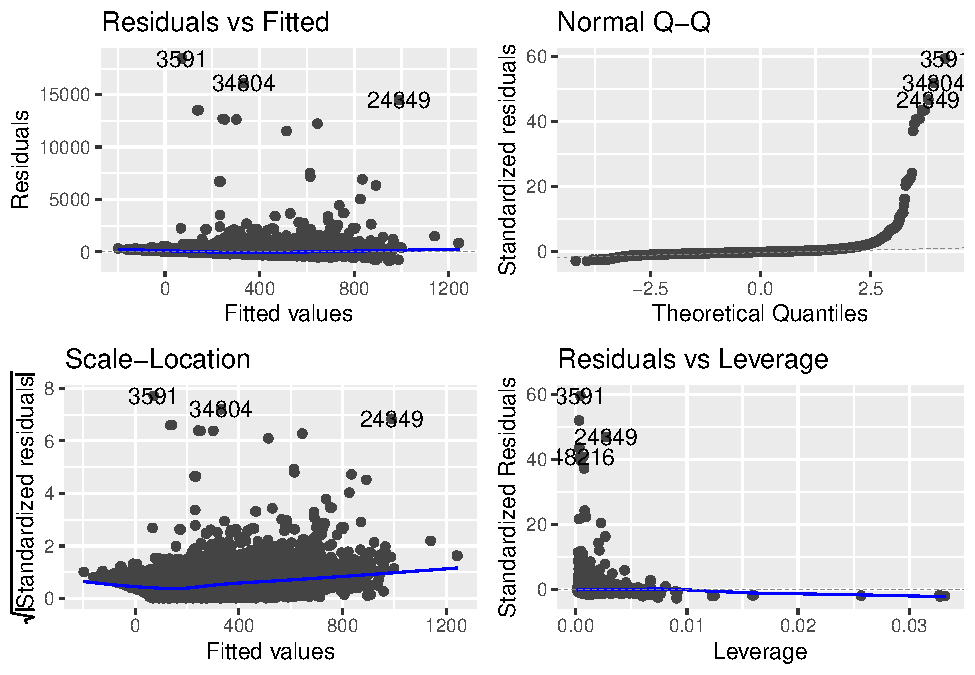
\includegraphics{Project_files/figure-latex/unnamed-chunk-24-1.pdf}

\begin{Shaded}
\begin{Highlighting}[]
\FunctionTok{autoplot}\NormalTok{(M1, }\AttributeTok{which =} \DecValTok{4}\NormalTok{)}
\end{Highlighting}
\end{Shaded}

\includegraphics{Project_files/figure-latex/unnamed-chunk-24-2.pdf}

\begin{Shaded}
\begin{Highlighting}[]
\FunctionTok{avPlots}\NormalTok{(M1)}
\end{Highlighting}
\end{Shaded}

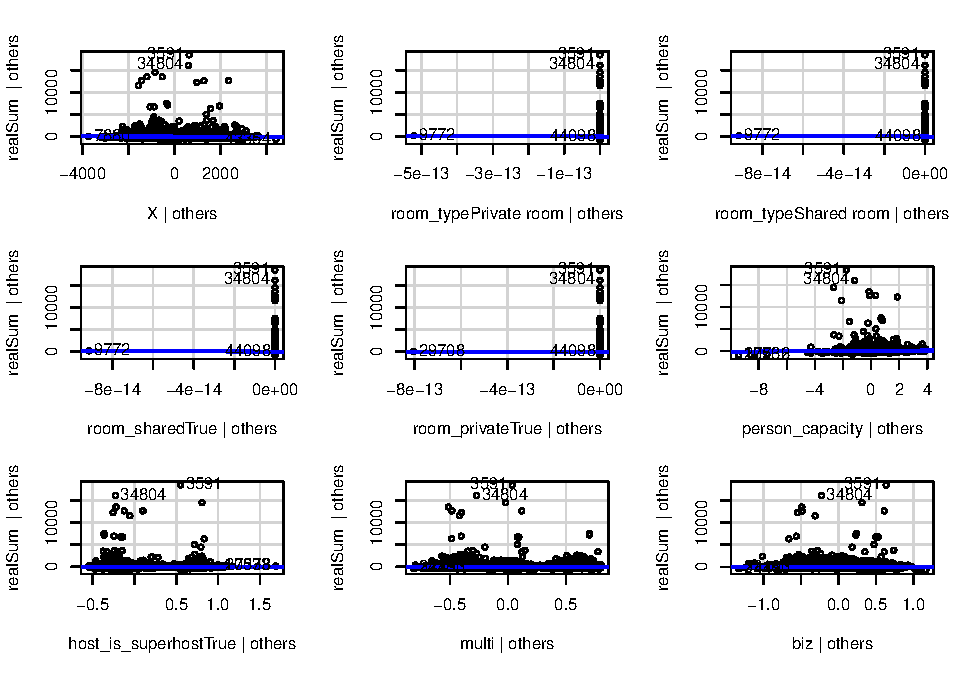
\includegraphics{Project_files/figure-latex/unnamed-chunk-24-3.pdf}
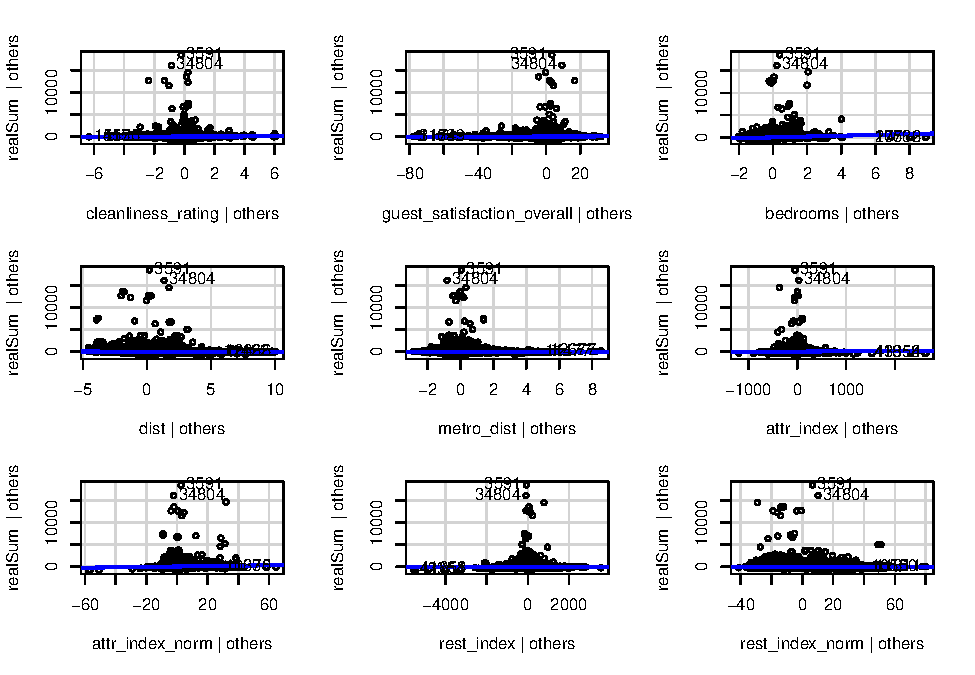
\includegraphics{Project_files/figure-latex/unnamed-chunk-24-4.pdf}
\includegraphics{Project_files/figure-latex/unnamed-chunk-24-5.pdf}

\hypertarget{cooks-distance}{%
\subsubsection{Cooks Distance}\label{cooks-distance}}

\begin{Shaded}
\begin{Highlighting}[]
\NormalTok{cooksd }\OtherTok{\textless{}{-}} \FunctionTok{cooks.distance}\NormalTok{(M1)}
\FunctionTok{max}\NormalTok{(cooksd)}
\end{Highlighting}
\end{Shaded}

\begin{verbatim}
## [1] 0.3151076
\end{verbatim}

\hypertarget{cooks-distance-v2}{%
\subsubsection{Cooks Distance V2}\label{cooks-distance-v2}}

\begin{Shaded}
\begin{Highlighting}[]
\NormalTok{augment\_M1 }\OtherTok{=} \FunctionTok{data.frame}\NormalTok{(}\FunctionTok{augment}\NormalTok{(M1))}
\FunctionTok{max}\NormalTok{(augment\_M1}\SpecialCharTok{$}\NormalTok{.cooksd)}
\end{Highlighting}
\end{Shaded}

\begin{verbatim}
## [1] 0.3151076
\end{verbatim}

\hypertarget{prediction-analysis}{%
\subsubsection{Prediction Analysis}\label{prediction-analysis}}

\begin{Shaded}
\begin{Highlighting}[]
\NormalTok{my\_data\_test\_spread }\OtherTok{\textless{}{-}}\NormalTok{ my\_data\_test }\SpecialCharTok{\%\textgreater{}\%}
    \FunctionTok{spread\_predictions}\NormalTok{(M1)}
\NormalTok{my\_data\_test\_spread }\OtherTok{\textless{}{-}}\NormalTok{ my\_data\_test }\SpecialCharTok{\%\textgreater{}\%}
    \FunctionTok{spread\_residuals}\NormalTok{(M1)}
\FunctionTok{mean}\NormalTok{(my\_data\_test\_spread}\SpecialCharTok{$}\NormalTok{M1)}
\end{Highlighting}
\end{Shaded}

\begin{verbatim}
## [1] -0.9869423
\end{verbatim}

\hypertarget{lasso-regression}{%
\subsection{Lasso Regression}\label{lasso-regression}}

\begin{Shaded}
\begin{Highlighting}[]
\NormalTok{x }\OtherTok{\textless{}{-}} \FunctionTok{as.matrix}\NormalTok{(my\_data[, }\FunctionTok{c}\NormalTok{(}\StringTok{"room\_type"}\NormalTok{, }\StringTok{"room\_shared"}\NormalTok{, }\StringTok{"room\_private"}\NormalTok{,}
    \StringTok{"person\_capacity"}\NormalTok{, }\StringTok{"host\_is\_superhost"}\NormalTok{, }\StringTok{"multi"}\NormalTok{, }\StringTok{"biz"}\NormalTok{, }\StringTok{"cleanliness\_rating"}\NormalTok{,}
    \StringTok{"guest\_satisfaction\_overall"}\NormalTok{, }\StringTok{"bedrooms"}\NormalTok{, }\StringTok{"dist"}\NormalTok{, }\StringTok{"metro\_dist"}\NormalTok{,}
    \StringTok{"attr\_index"}\NormalTok{, }\StringTok{"attr\_index\_norm"}\NormalTok{, }\StringTok{"rest\_index"}\NormalTok{, }\StringTok{"rest\_index\_norm"}\NormalTok{,}
    \StringTok{"lng"}\NormalTok{, }\StringTok{"lat"}\NormalTok{, }\StringTok{"city\_day"}\NormalTok{)])}
\NormalTok{y }\OtherTok{\textless{}{-}}\NormalTok{ my\_data}\SpecialCharTok{$}\NormalTok{realSum}
\NormalTok{lasso.fit }\OtherTok{\textless{}{-}} \FunctionTok{glmnet}\NormalTok{(x, y, }\AttributeTok{alpha =} \DecValTok{1}\NormalTok{)}
\FunctionTok{plot}\NormalTok{(lasso.fit, }\AttributeTok{xvar =} \StringTok{"lambda"}\NormalTok{, }\AttributeTok{label =} \ConstantTok{TRUE}\NormalTok{)}
\end{Highlighting}
\end{Shaded}

\includegraphics{Project_files/figure-latex/unnamed-chunk-28-1.pdf}

\hypertarget{model-selection}{%
\section{Model Selection}\label{model-selection}}

\hypertarget{model-training}{%
\section{Model Training}\label{model-training}}

\hypertarget{conclusion}{%
\section{Conclusion}\label{conclusion}}

\end{document}
